\documentclass[../main/TimeForcingSHE.tex]{subfiles} 
\begin{document}


\section{Persistence of defects due to oscillations}
\subsection{show solutions of quasistable defect connecting to both 39 and 40 period solution as well as stable defect}
\subsection{graph of regions where for each case}
\subsection{Some kind of explanaition (Eckaus instability and delayed bifurcations?)}

Using an oscillation with a period of 50 and centered about $r_0=-0.27$ and amplitude of $\rho =0.1$, we can see the trajectory taken by the initial localized solution as it approaches a domain filling one (Fig.~\ref{fig:FillDomain}).  The solution grows by nucleating a period on each front at each oscillation of the forcing parameter. This happens until the solution reaches 39 periods, at which point it seems to get stuck.  Eventually it fills the domain with a 40 period solution.  This is in contrast to the case with a constant forcing that grows into the domain with a 39 period solution.  

\begin{figure}[h]
  \begin{center}
    \mbox{
      \subfloat[]{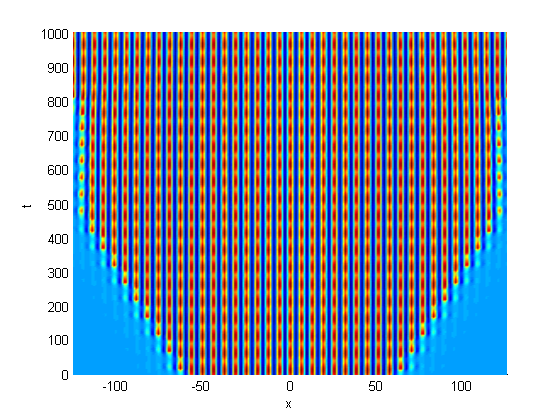
\includegraphics[width=60mm]{r0nD270drD10t050sol.png}} \quad
      \subfloat[]{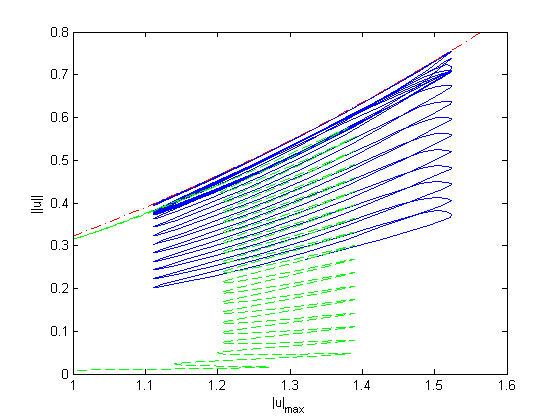
\includegraphics[width=60mm]{r0nD270drD10t050phase.png} }
      }
    \caption{Oscillations of the forcing parameter in and out of the snaking region.  The forcing parameter as a function of time is given by $r\rightarrow -0.27+ 0.1\sin2\pi t/50$.  The solution (a) grows in time, eventually filling the domain and the corresponding trajectory along the max value - L2 norm phase space slice (b) shows the path taken as it passes in and out of the snaking region . }
    \label{fig:FillDomain}
  \end{center}
\end{figure} 


\end{document}